%\documentclass[handout]{beamer}
\documentclass[ignorenonframetext]{beamer}
\usepackage{textpos}
\usepackage{graphicx}
\usepackage{pgf}
\usepackage{caption}
\usepackage{listings}
\usepackage{multimedia}
\usepackage{gensymb}
\usepackage{amsmath, mathrsfs}

% \captionsetup[figure]{labelformat=empty}% redefines the caption setup of the figures environment in the beamer class.

\usetheme{Boadilla}
\usefonttheme{serif}
% \mode<presentation>
% {
%  \usefonttheme{serif}
% % \useoutertheme{sidebar}
% %   \logo{\includegraphics[height=1cm]{elec_logo.pdf}}
% }

\title[TART]{BIUST Workshop Outcome: Research Projects}
\author[Molteno]{Tim Molteno}

\institute[Otago]
{
  Electronics Research Foundation \\
  \& \\
  Department of Physics,
  University of Otago \\
  \vspace{1cm}
  \large{Dunedin, New Zealand.}\\
  \vspace{2cm}
  \includegraphics[width=0.6\linewidth]{../tart_overview/fig/elec_header_font.pdf}
}

\logo{\pgfputat{\pgfxy(-0.72,7.7)}{\pgfbox[center,base]{\includegraphics[width=1cm]{../tart_overview/fig/elec_logo.pdf}}}}

\date[BIUST 03/2025] % (optional, should be abbreviation of conference name)
{}

\begin{document}

% Abstract: In this talk I'll give an overview of Africa's newest radio telescope, the TART, recently installed in Mauritius in a joint effort between SARAO, the University of Otago (NZ). I'll talk about TARTs origins, it's design and open-source philosophy as well as the upcoming project to install TART telescopes in the SKA African partner nations. I'll also include some details about improvements that will appear in TART-3, the next version of TART!

\begin{frame}
  \titlepage
\end{frame}
 
\begin{frame}
\vspace{1cm}

  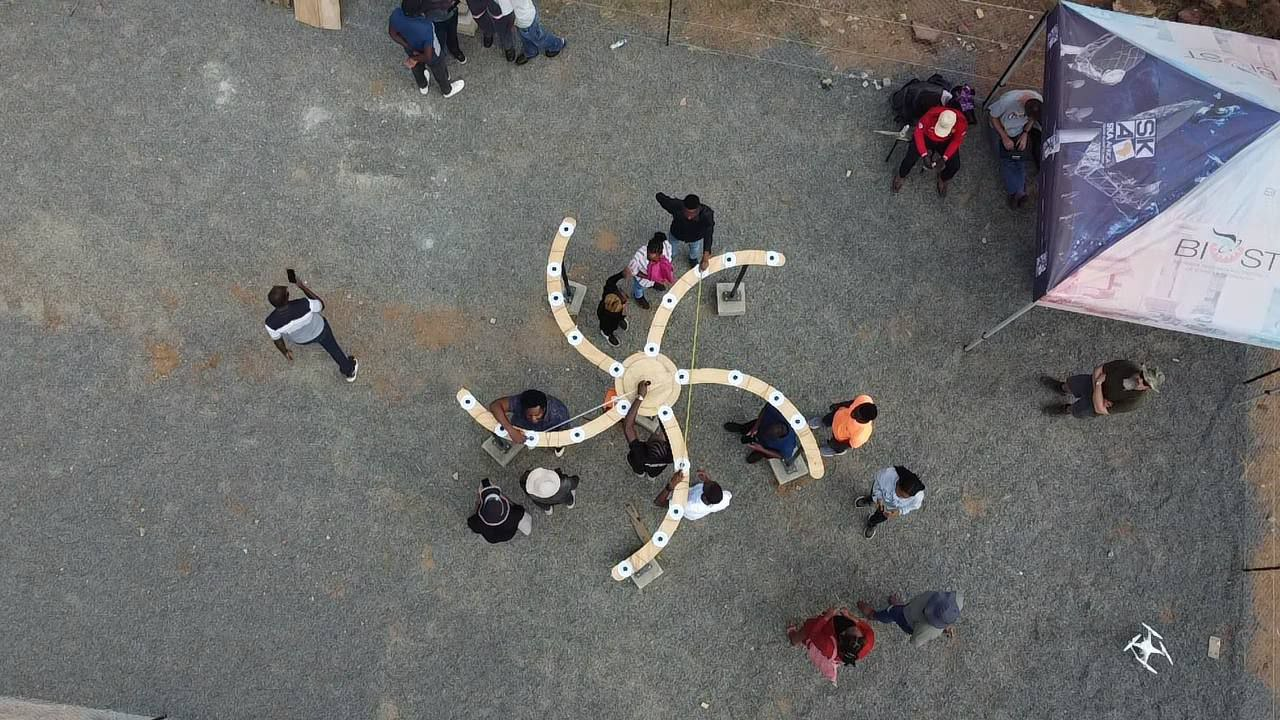
\includegraphics[width=\linewidth]{fig/biust_from_above.jpg}\\
  \centering{BIUST TART final calibration. Yesterday!}
\end{frame}

% \begin{frame}{Abstract}
%  I will introduce the Transient Array Radio Telescope. Developed here in the Department of Physics at Otago University, this is the worlds smallest (and cheapest) aperture synthesis radio telescope -- that is a telescope that creates images of the radio sky. It is now being used by astronomers working on the Square Kilometer Array, the worlds largest radio telescope -- as an instrument that can be used to both develop new algorithms for radio astronomy and also to teach students about how radio telescopes work. I will describe the instrument and how it works, as well as giving an overview of the upcoming projects involving this telescope in Africa.
% \end{frame}

\begin{frame}
  \tableofcontents
  % You might wish to add the option [pausesections]
\end{frame}

\section{Potential Projects}


\begin{frame}{Potential Projects}
 \begin{columns}
  \begin{column}{0.6\linewidth}
    \begin{itemize}
    \item Will require a BIUST supervisor.
    \item Could use a remote supervisor.
    \item SARAO / DARA scholarships may be available
    \end{itemize}
  \end{column}
  \begin{column}{0.4\linewidth}
    \includegraphics[width=\linewidth]{fig/tart3.jpg}
  \end{column}
\end{columns}
\end{frame}



\subsection{Automatic Tracking of Near Earth Objects}
\begin{frame}{Automatic Tracking}
\begin{center}
\includegraphics[width=0.8\linewidth]{fig/elaz.jpg}\\
 Consistent with something in low-earth orbit.
 \end{center}
  \begin{block}{Remote Supervisors}
 Ben or Tim
 \end{block}

\end{frame}


\subsection{Explore new imaging ideas}
\begin{frame}{New imaging ideas}
\begin{center}
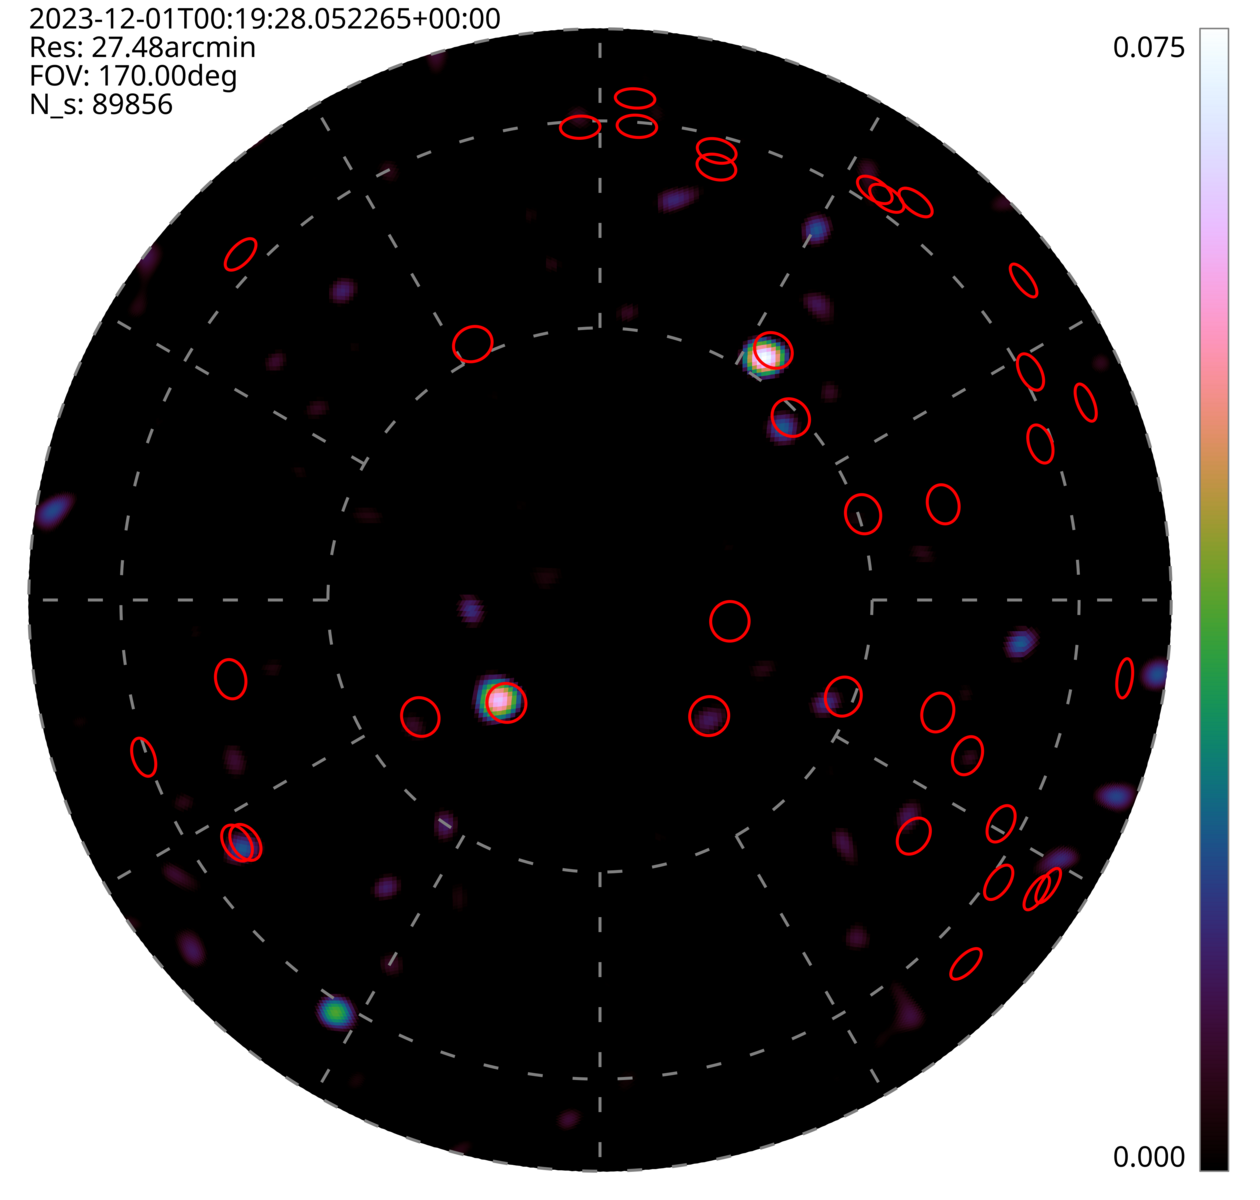
\includegraphics[width=0.7\linewidth]{../tart_imaging/images/obs_00000.hdf.png}
 \end{center}
  \begin{block}{Remote Supervisors}
 Oleg, Ben or Tim
 \end{block}
\end{frame}



\subsection{Machine Learning and Imaging}
\begin{frame}{Machine Learning and imaging}
\begin{center}
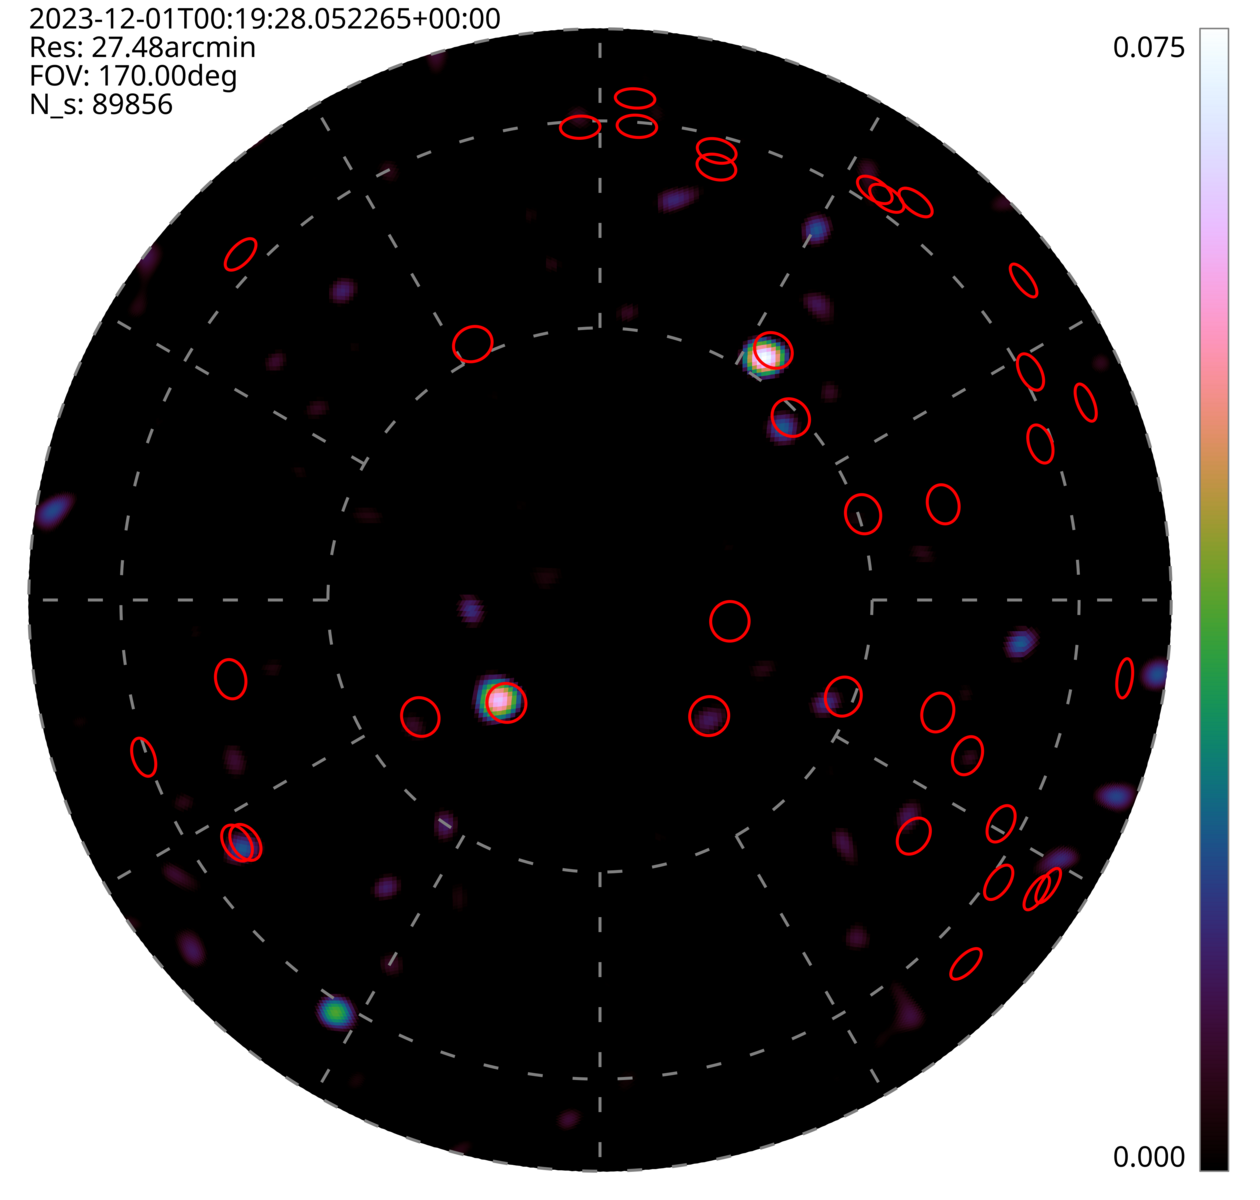
\includegraphics[width=0.5\linewidth]{../tart_imaging/images/obs_00000.hdf.png}
 \end{center}
 Use machine learning frameworks to learn how to create images from visibility data.

 \begin{block}{Remote Supervisors}
 Oleg, Ben or Tim
 \end{block}
\end{frame}



\section{New Antennas}
\begin{frame}{New TART Antenna Designs}
\begin{center}
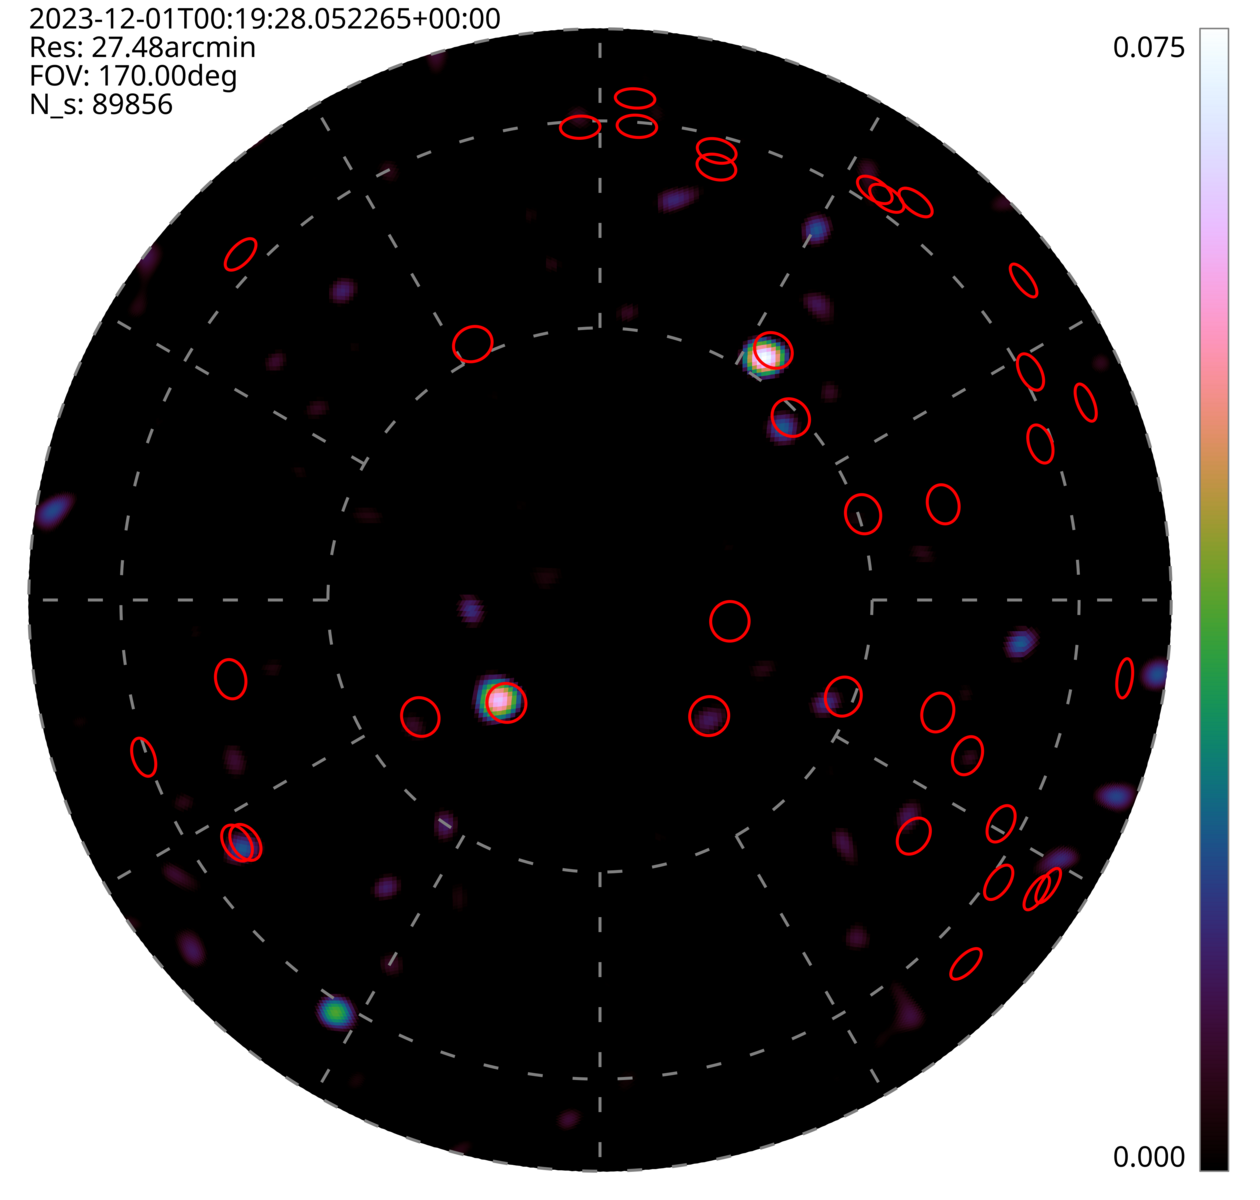
\includegraphics[width=0.5\linewidth]{../tart_imaging/images/obs_00000.hdf.png}
 \end{center}
Develop new antenna designs
 \begin{block}{Remote Supervisors}
 EMSS, Rhodes, Tim
 \end{block}
\end{frame}


\subsection{Better array calibration}

\begin{frame}{Better position calibration}
\begin{center}
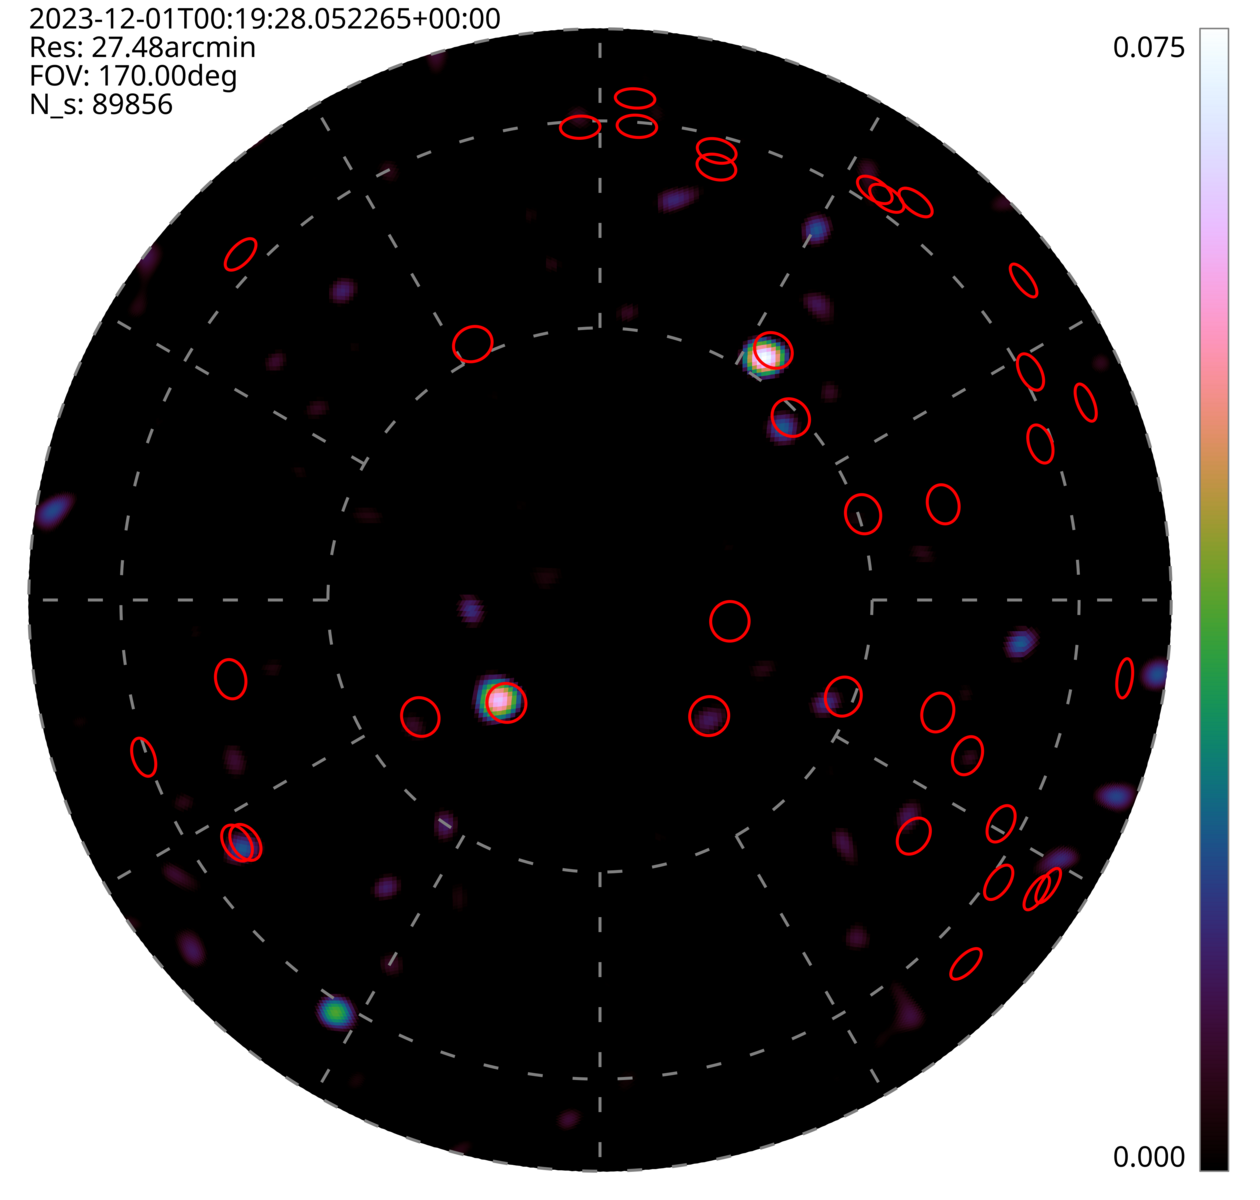
\includegraphics[width=0.5\linewidth]{../tart_imaging/images/obs_00000.hdf.png}
 \end{center}
Drones, new code e.t.c
 \begin{block}{Remote Supervisors}
 Ben, Tim
 \end{block}
\end{frame}


\subsection{Searching for transients}

\begin{frame}{Searching for transients}
\begin{center}
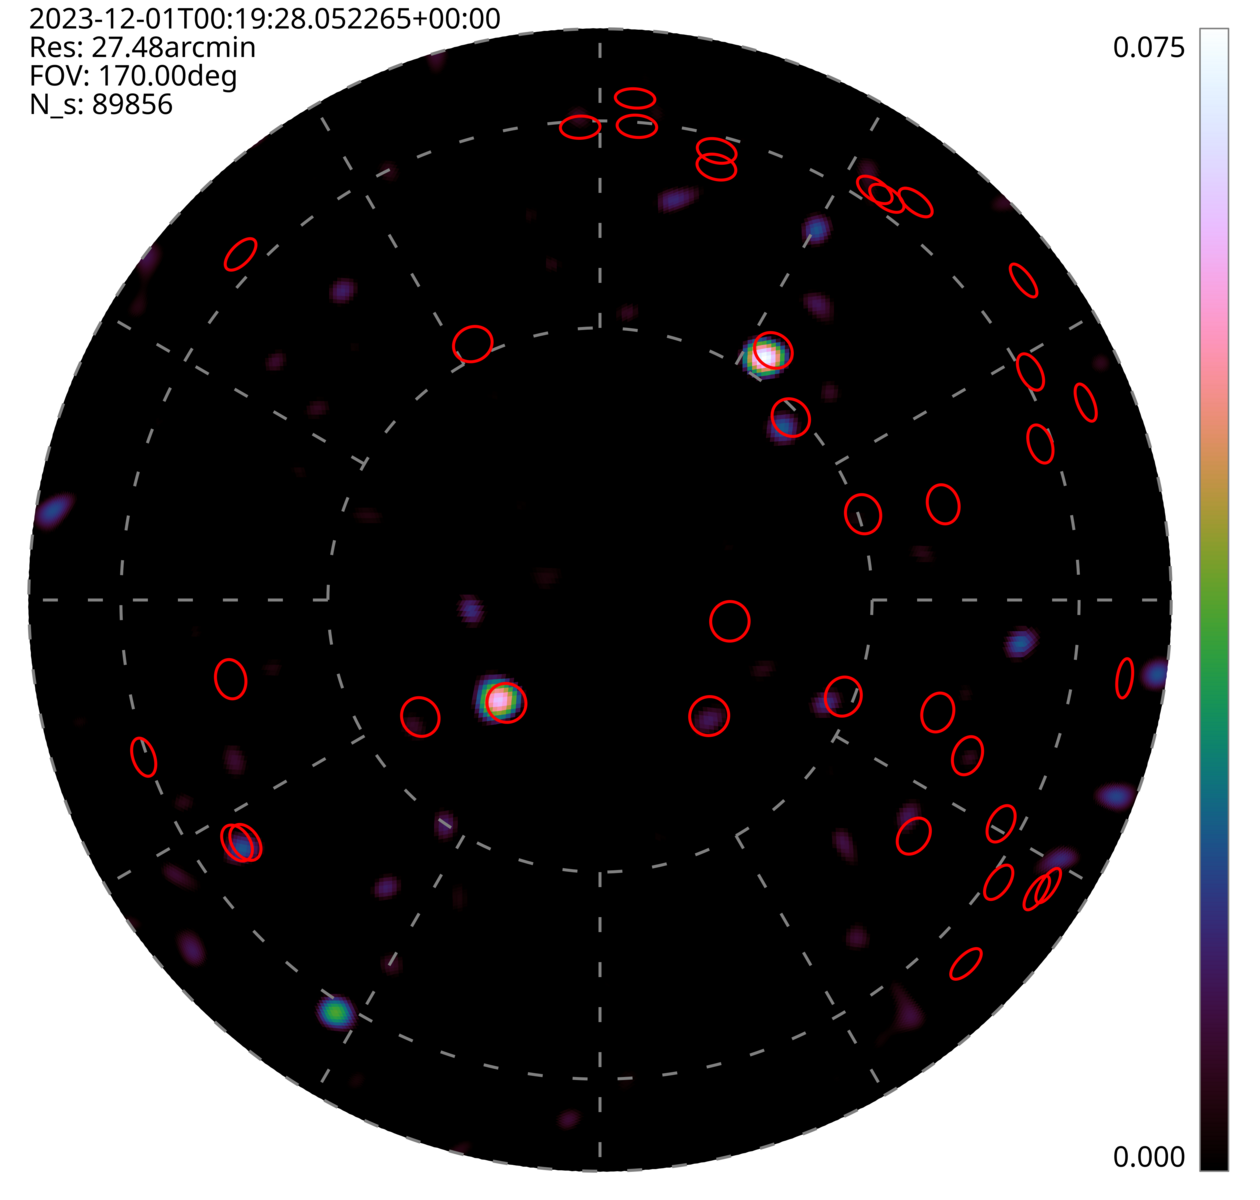
\includegraphics[width=0.5\linewidth]{../tart_imaging/images/obs_00000.hdf.png}
 \end{center}
Drones, new code e.t.c
 \begin{block}{Remote Supervisors}
 Many available, SARAO, Rhodes e.t.c.
 \end{block}
\end{frame}



\end{document}
